\section{Energy Ridges}
\label{al-energy-ridges}



\bit
\item 2 concerted "gateway" between hop and other concerted motion.
\eit



\placeholder


\begin{comment}
--- Anything below here is a direct copy from either the \latex file of the manuscript or the online version of the article ---

\section{\label{sec:results-adatom}Application: Al adatom diffusion on an Al(100) surface}

An Al adatom on the Al(100) surface provides an interesting system to study because several different diffusion mechanisms have been found, including various concerted displacements of two or more atoms, in addition to the, more intuitive, hop mechanism~\cite{concerted-motion-1990, dimer-original-1999, johannessson-01}.
An embedded atom method potential (EAM)~\cite{eam-1986} is used here since it has been shown to accurately describe the system and requires much less computational effort than DFT calculations.
The simulated cell was a slab of 6 layers, each of which was $8\times8$ atoms, with one adatom, totalling 385 atoms.
The two bottom layers were kept fixed at bulk positions with a lattice parameter of $4.038\unit{\mAA}$.
Initially, traditional NEB calculations were carried out to find the relevant \sap{1}s which were then used as end points in the ridge calculations.
The spring constant was set at $k = 5.0\unit{eV/\mAA}$.
The two images in the dimer had a fixed separation of $0.0001\unit{\mAA}$ and were allowed to rotate only once for each iteration in the path optimisation.
The initial minimum mode guesses were taken from a Gaussian distribution.
The convergence criteria for the maximum effective force component were set at $0.01\unit{eV/\mAA}$ and $0.001\unit{eV/\mAA}$ for the regular and climbing image calculations respectively.

% Figure 4
\begin{figure}[t]
\begin{center}
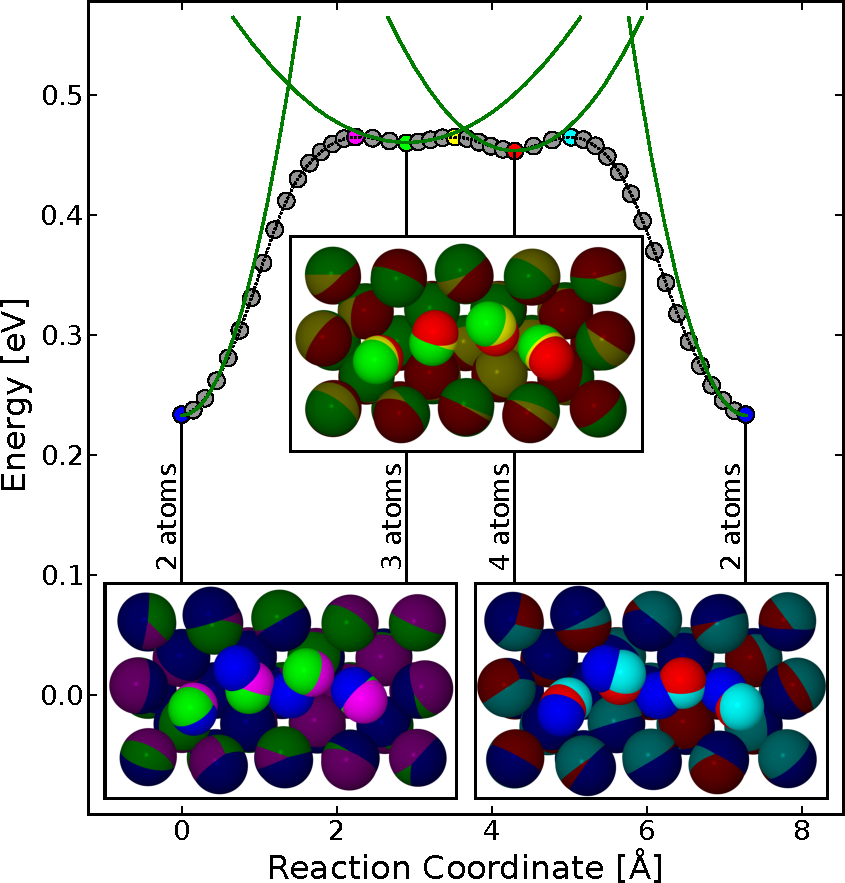
\includegraphics[width=0.5\linewidth]{figures/low-barriers}
\caption{
The energy ridge going through \sap{1}s of 2-atom, 3-atom, 4-atom and, then the same, 2-atom concerted displacement for an Al adatom on a Al(100) surface.
The circles represent the position of images in the optimised paths, the \sap{1}s and the \sap{2}s being coloured differently but the rest coloured grey.
The green curves represent harmonic approximations to the energy surface at each \sap{1}.
The insets show an overlay of three configurations, two adjacent \sap{1}s and the intermediate \sap{2}.
The atom colours correspond to the coloured spheres of the energy ridge.
The \sap{2}s adjacent to the 3-atom and 4-atom concerted displacements are low and the harmonic approximation to TST is less accurate for these mechanisms than the 2-atom concerted displacement.
}
\label{fig:low-barriers}
\end{center}
\end{figure}

Several low energy transition mechanisms for adatom diffusion on this surface have been found previously using the dimer method \cite{dimer-original-1999}.
The mechanism with the lowest energy barrier is a two atoms concerted displacement, $E_b = 0.227\unit{eV}$.
The second lowest is the simple hop of the adatom from one site to an adjacent site, $E_b = 0.372\unit{eV}$, but then three and four atoms concerted displacements are only slightly higher in energy $E_b = 0.426\unit{eV}$ and $E_b = 0.413\unit{eV}$.

The potential energy ridges and \sap{2}s were calculated between each pair of \sap{1}s and the results are shown in \fref{fig:low-barriers} for the three concerted displacement mechanisms.
Low energy \sap{2}s were found near the concerted 3- and 4- atom displacement \sap{1}s, with energy $\mytilde0.005\unit{eV}$ and $\mytilde0.012\unit{eV}$.
The energy of these \sap{2}s is less than thermal energy at room temperature, $k_\text{B}T = 0.025\unit{eV}$, over the adjacent \sap{1}s,
which means that HTST is likely not a good approximation for these mechanisms.

In principle, knowledge of the ridge and the \sap{2}s can be used to improve on the HTST approximation.
Here, a rough estimate of a correction factor, $\Gamma$, will be evaluated by calculating the ratio of the configuration integrals of the harmonic approximation to that calculated from the potential energy along the ridge,
\begin{equation}
\Gamma \ = \ \frac{Z^{ridge}_\ddagger}{Z^{harm}_\ddagger} \ = \  \frac{\int_{ridge} \exp[-E(x)/k_\text{B}T] dx}{\int_{-\infty}^\infty \exp[-\alpha x^2 / k_\text{B}T]dx} \ ,
\label{eq:harmonic-correction-factor}
\end{equation}
where $x$ is the displacement along the ridge and $\alpha$ is the curvature of the one-dimensional parabola obtained by performing least squares analysis of the 4 images closest to the \sap{1}s.
The ratios obtained with \eref{eq:harmonic-correction-factor} are shown as a function temperature in \fref{fig:integral-ratios}.
As expected, the harmonic approximation works well for the concerted 2-atom process as the \sap{1} is much lower in energy than the adjacent \sap{2}s in that case.
On the other hand the concerted 3- and 4-atom displacements have a significant correction factor ($\mytilde0.5$ for the concerted 4-atom process at $350\unit{K}$) as can be seen from the figure.
It should be noted that the ratio increases with temperature due to the limited range of the ridge integral as compared with the infinite limits of the harmonic one.
This is particularly prominent for the 2-atom concerted displacement where the ratio even goes above $1.0$.
In high dimensional systems, \sap{1}s lie on multiple ridges, as can be seen in figure \fref{fig:multiple-ridges},
where 3 of the different ridges which the concerted 2-atom displacement \sap{1} lies on, are shown.
Thus it may be necessary to perform corrections such as those above for more than one ridge for any given \sap{1}.

% Figure 5
\begin{figure}[t]
\begin{center}
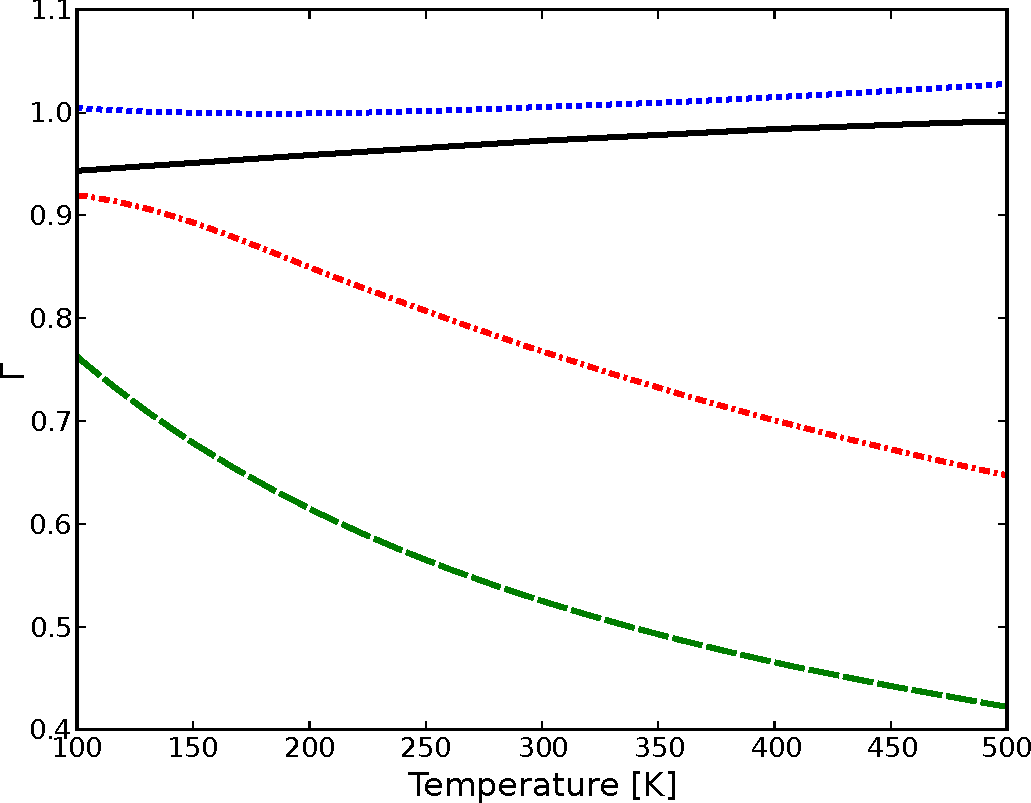
\includegraphics[width=0.5\linewidth]{figures/integral-ratios}
\caption{
The ratio, $\Gamma$, defined in \eref{eq:harmonic-correction-factor},
between the configuration integrals of the potential energy ridge shown in \fref{fig:low-barriers} and the corresponding harmonic approximations.
The black, solid, line is the ratio for the full integral, including all three concerted displacement processes.
The blue, dotted, line is the ratio when only considering the 2-atom concerted displacement.
The green, dashed, line is the ratio when only considering the 3-atom concerted displacement.
The red, dash-dotted, line is the ratio when only considering the 4-atom concerted displacement.
For the individual processes, the end points of the ridge integral are the adjacent \sap{2}s, while the full integral is done for the whole ridge.
While the harmonic approximation gives a good approximation for the total configuration integral over the whole temperature range shown, because it is dominated by the 2-atom displacement, the estimate for each of the 3-atom and 4-atom displacements is poor unless the temperature is very low.
}
\label{fig:integral-ratios}
\end{center}
\end{figure}
% ----------------------------

In the insets of \fref{fig:low-barriers}, a comparison of the atom coordinates at two adjacent \sap{1} and the intermediate \sap{2} can be seen.
In particular, the difference between the concerted 3- and 4-atom \sap{1}s is shown.
The coordinates of the two left-most atoms only change slightly while the two right-most coordinates change more, as is to be expected as the atom furthest to the right is not directly involved in the concerted 3-atom process.
The similarities in coordinates and the small \sap{2}s separating the 3- and 4-atom displacement processes indicate that a trajectory passing through the vicinity of either \sap{1} could easily end up on the product state corresponding to the other.
Dynamical trajectories started at the ridge would be needed to determine the probability of each of the product states.

% Figure 6
\begin{figure}[t]
\begin{center}
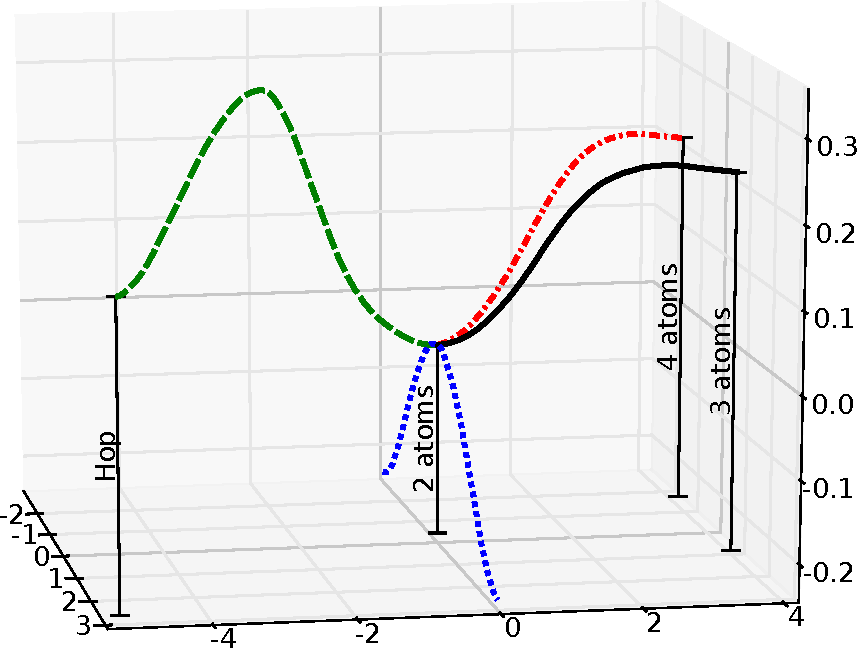
\includegraphics[width=0.5\linewidth]{figures/many-ridges}
\caption{
A schematic view (due to the high dimensionality of the system) of some of the ridges lying through the \sap{1} for 2-atom concerted displacement (the MEP is shown with blue dotted line).
The three ridges shown connect to the \sap{1}s of the hop and the 2-atom and 3-atom displacements mechanisms
The vertical bars represent the height of each of the \sap{1}s.
The figure illustrates that a \sap{1} typically lies on several energy ridges for a complex system.
}
\label{fig:multiple-ridges}
\end{center}
\end{figure}

When finding the ridge between the concerted 4-atom displacement and the hop \sap{1}s,
shown in \fref{fig:barriers-discovery},
it became apparent that a ridge does not directly connect the two.
Instead, the ridge passes through the concerted 2-atom displacement \sap{1}.
The path passes exactly through the highest \sap{2}, 
as can be verified from the calculated force, given that the climbing image algorithm is employed.
However, due to the possible corner cutting, there is no guarantee that other, lower energy, \sap{2}s along the ridge will be found exactly.
Nevertheless, if a sufficient number of images is used,
the path will give good approximation for any \sap{1}s and \sap{2}s along the ridge.
Here, the image closest to the concerted 2-atom displacement \sap{1} is found to be at a $0.004\unit{\mAA/\text{atom}}$ distance from the exact \sap{1}.
Using these coordinates in a \sap{1} searching algorithm quickly yields the exact \sap{1}.
As for the lower \sap{2}, a second ridge calculation can be performed with the adjacent \sap{1}s as endpoints to focus on a shorter segment of the ridge with only one intermediate \sap{2},
thereby enabling the climbing image to converge exactly on the lower \sap{2}.
This is shown in \fref{fig:barriers-discovery}, where the discovered \sap{1} is used as an endpoint in a subsequent optimisation of a shorter path and, thus, the lower \sap{2} is found accurately.

% Figure 7
\begin{figure}[b]
\begin{center}
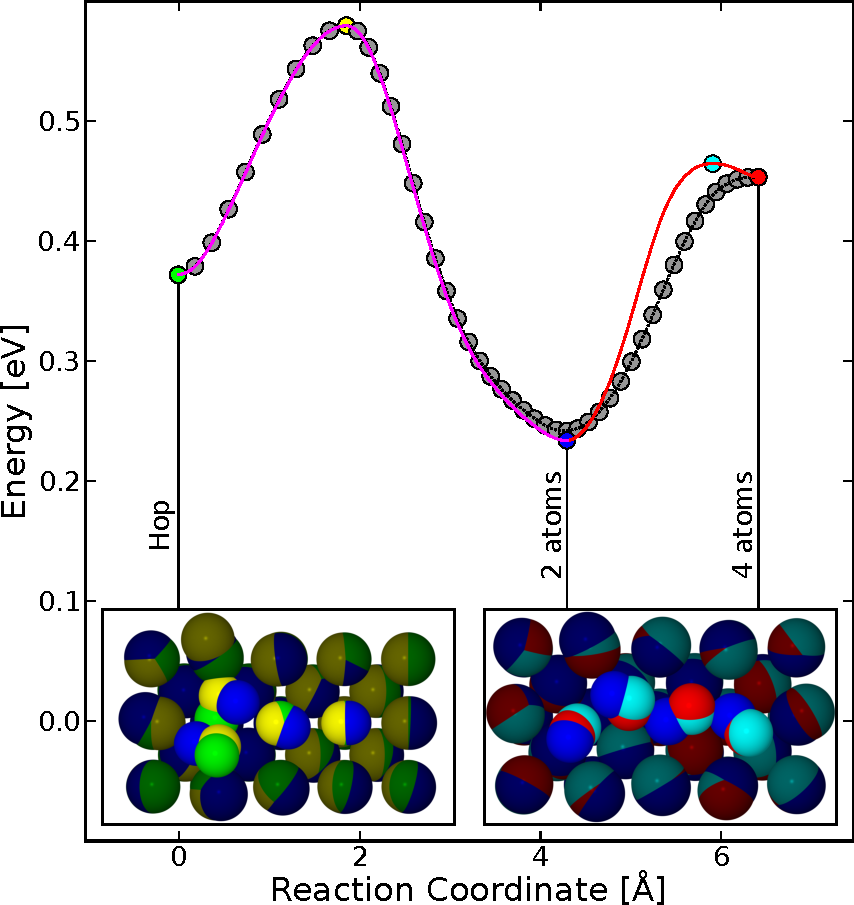
\includegraphics[width=0.5\linewidth]{figures/discovery}
\caption{
Calculated path at the ridge between the \sap{1}s for a hop and concerted 4-atom displacement.
The circles show the position of converged images (coloured circles for \sap{1}s and \sap{2}s, but gray for the rest). 
These \sap{1}s turned out not to be adjacent on a ridge and the path optimisation reveals an intermediate \sap{1}, the one for the concerted 2-atom displacement.
This illustrates how a ridge calculation could reveal new and possibly unknown transition mechanisms.
The long path is not able to accurately locate the intermediate \sap{1} and the lower energy \sap{2} due to finite resolution in the discretisation and corner-cutting.
The exact configuration of the \sap{1} can be found using a \sap{1} finding algorithm starting with the approximation obtained from the optimised path.
Then, a calculation of a shorter path, between the \sap{1}s of the 2-atom  and 4-atom displacements, locates the intermediate \sap{2} accurately (cyan circle)
The insets show an overlay of three configurations, two adjacent \sap{1}s and the intermediate \sap{2}.
The atom colours correspond to the coloured spheres of the energy ridge.
}
\label{fig:barriers-discovery}
\end{center}
\end{figure}
\end{comment}
